%! Author = Len Washington III
%! Date = 10/02/2023

% Preamble
\documentclass[title={Oct 02, 2023 Notes}]{math252notes}

% Document
\begin{document}

\setcounter{chapter}{4}
\chapter[Modeling with Higher-Order DEs]{Modeling with Higher-Order Differential Equations}\label{ch:modeling-with-higher-order-differential-equations}
\setcounter{section}{0}
\section{Spring-Mass Problems}\label{sec:spring-mass-problems}
\subsubsection{Last Time}\label{subsec:last-time} If you have free, undamped motion, where your point of equilibrium is $x=0$ and the downward direction is positive:

%<*Section-5.1-2>
\subsection{Undamped Motion}\label{subsec:undamped-motion}
\begin{equation*}
\begin{aligned}
	m\frac{d^{2}x}{dt^{2}} + kx &= 0\\
	\frac{d^{2}x}{dt^{2}} + \frac{k}{m}x &= 0\\
	\frac{d^{2}x}{dt^{2}} + \omega^{2}x &= 0 \mbox{ where }\omega = \sqrt{\frac{k}{m}}\\
	n^{2}e^{nt} + \omega^{2}e^{nt} &= 0 \mbox{ where } x = e^{nt}\\
	n^{2} + \omega^{2} &= 0 \\
	n^{2} &= -\omega^{2} \\
	n &= 0\pm\sqrt{-\omega^{2}} \\
	  &= 0\pm\omega i \\
\end{aligned}
\end{equation*}
\begin{equation*}
\begin{aligned}
	x_{1} = \cos(\omega t) \sep x_{2} = \sin(\omega t)\\
\end{aligned}
\end{equation*}
General solution:\label{eq:spring-mass-general-solution} \[ x = c_{1}\cos(\omega t) + c_{2}\sin(\omega t)\\ \]

\subsection{Free, Damped Motion}\label{subsec:free-damped-motion}
Assume in addition to $F_{spring}$ and $F_{gravity}$ that there is a force damping the motion which is directly proportional, in the opposite direction, to the mass's velocity.

\begin{equation}
\begin{aligned}
	m\frac{d^{2}x}{dt^{2}} + \beta\frac{dx}{dt} + kx &= 0\\
	\frac{d^{2}x}{dt^{2}} + \frac{\beta}{m}\frac{dx}{dt} + \frac{k}{m}x &= 0\\
	\frac{d^{2}x}{dt^{2}} + \frac{\beta}{m}\frac{dx}{dt} + \omega^{2}x &= 0\\
\end{aligned}
\end{equation}
where $\beta$ is the drag coefficient. If we substitute $2\lambda = \frac{\beta}{m} \Rightarrow \lambda = \frac{\beta}{2m}$
\begin{equation*}
\begin{aligned}
	\frac{d^{2}x}{dt^{2}} + 2\lambda\frac{dx}{dt} + \omega^{2}x &= 0\\
	n^{2}e^{nt} + 2\lambda ne^{nt} + \omega^{2}e^{nt} &= 0\\
	n^{2} + 2\lambda n + \omega^{2} &= 0\\
	n^{2} + 2\lambda n &= -\omega^{2} \\
	n^{2} + 2\lambda n + \lambda^{2} &= \lambda^{2} - \omega^{2} \\
	(n + \lambda)^{2} &= -\omega^{2} + \lambda^{2} \\
	n + \lambda &= \pm\sqrt{\lambda^{2} - \omega^{2}} \\
	n &= -\lambda \pm\sqrt{\lambda^{2} - \omega^{2}} \\
\end{aligned}
\end{equation*}

\subsubsection{Case 1: $\lambda^{2} > \omega^{2}$}\label{subsubsec:spring-mass-case-1} then there are two distinct real solutions where $n_{1} < 0$ and $n_{2} < 0$.
\begin{equation*}
\begin{aligned}
	n_{1} &= -\lambda + \sqrt{\lambda^{2} - \omega^{2}}\\
	n_{2} &= -\lambda - \sqrt{\lambda^{2} - \omega^{2}}\\
\end{aligned}
\end{equation*}\begin{equation*}
\begin{aligned}
	x_{1} = e^{n_{1}t} \sep x_{2} = e^{n_{2}t}\\
	x_{1} = e^{t\left( -\lambda + \sqrt{\lambda^{2} - \omega^{2}} \right)} \sep x_{2} = e^{t\left( -\lambda - \sqrt{\lambda^{2} - \omega^{2}} \right)}\\
\end{aligned}
\end{equation*}
General solution: \begin{equation}
\begin{aligned}
	x &= c_{1}e^{t\left( -\lambda + \sqrt{\lambda^{2} - \omega^{2}} \right)} + c_{2}e^{t\left( -\lambda - \sqrt{\lambda^{2} - \omega^{2}} \right)}\\
	  &= c_{1}e^{-t\lambda}e^{t\sqrt{\lambda^{2} - \omega^{2}} } + c_{2}e^{-t\lambda}e^{-t\sqrt{\lambda^{2} - \omega^{2}}}\\
	  &= e^{-\lambda t}\left( c_{1}e^{t\sqrt{\lambda^{2} - \omega^{2}} } + c_{2}e^{-t\sqrt{\lambda^{2} - \omega^{2}}} \right)\\
\end{aligned}\label{eq:spring-case-1}
\end{equation}

\subsubsection{Case 2: $\lambda = \omega$}\label{subsubsec:spring-mass-case-2}
\begin{equation*}
\begin{aligned}
	n &= -\lambda \pm\sqrt{\lambda^{2} - \omega^{2}}\\
	n &= -\lambda \pm\sqrt{0}\\
	n &= -\lambda \\
\end{aligned}
\end{equation*} where $\lambda$ has multiplicity 2.
\begin{equation*}
\begin{aligned}
	x_{1} = e^{-\lambda t} \sep x_{2} = te^{-\lambda t}
\end{aligned}
\end{equation*}
General solution:
\begin{equation}
\begin{aligned}
	x &= c_{1}e^{-\lambda t} + c_{2}te^{-\lambda t}\\
	  &= e^{-\lambda t}\left( {1} + c_{2}t \right)\\
\end{aligned}\label{eq:spring-case-2}
\end{equation}

\subsubsection{Case 3: $\lambda^{2} < \omega^{2}$}\label{subsubsec:spring-mass-case-3} then
\begin{equation*}
\begin{aligned}
	x_{1} = e^{-\lambda t}\cos\left( \sqrt{\omega^{2} - \lambda^{2}}t \right) \sep x_{2} = e^{-\lambda t}\sin\left( \sqrt{\omega^{2} - \lambda^{2}}t \right)\\
\end{aligned}
\end{equation*}
\begin{equation}
\begin{aligned}
	x &= c_{1}e^{-\lambda t}\cos\left( \sqrt{\omega^{2} - \lambda^{2}}t \right) + c_{2}e^{-\lambda t}\sin\left( \sqrt{\omega^{2} - \lambda^{2}}t \right)\\
	  &= e^{-\lambda t}\left( c_{1}\cos\left( \sqrt{\omega^{2} - \lambda^{2}}t \right) + c_{2}\sin\left( \sqrt{\omega^{2} - \lambda^{2}}t \right) \right)\\
	  &= e^{-\lambda t}\left( A\sin\left( \sqrt{\omega^{2} - \lambda^{2}}t \right) + \phi \right)\\
\end{aligned}\label{eq:spring-case-3}
\end{equation}

\begin{figure}[H]
	\centering
	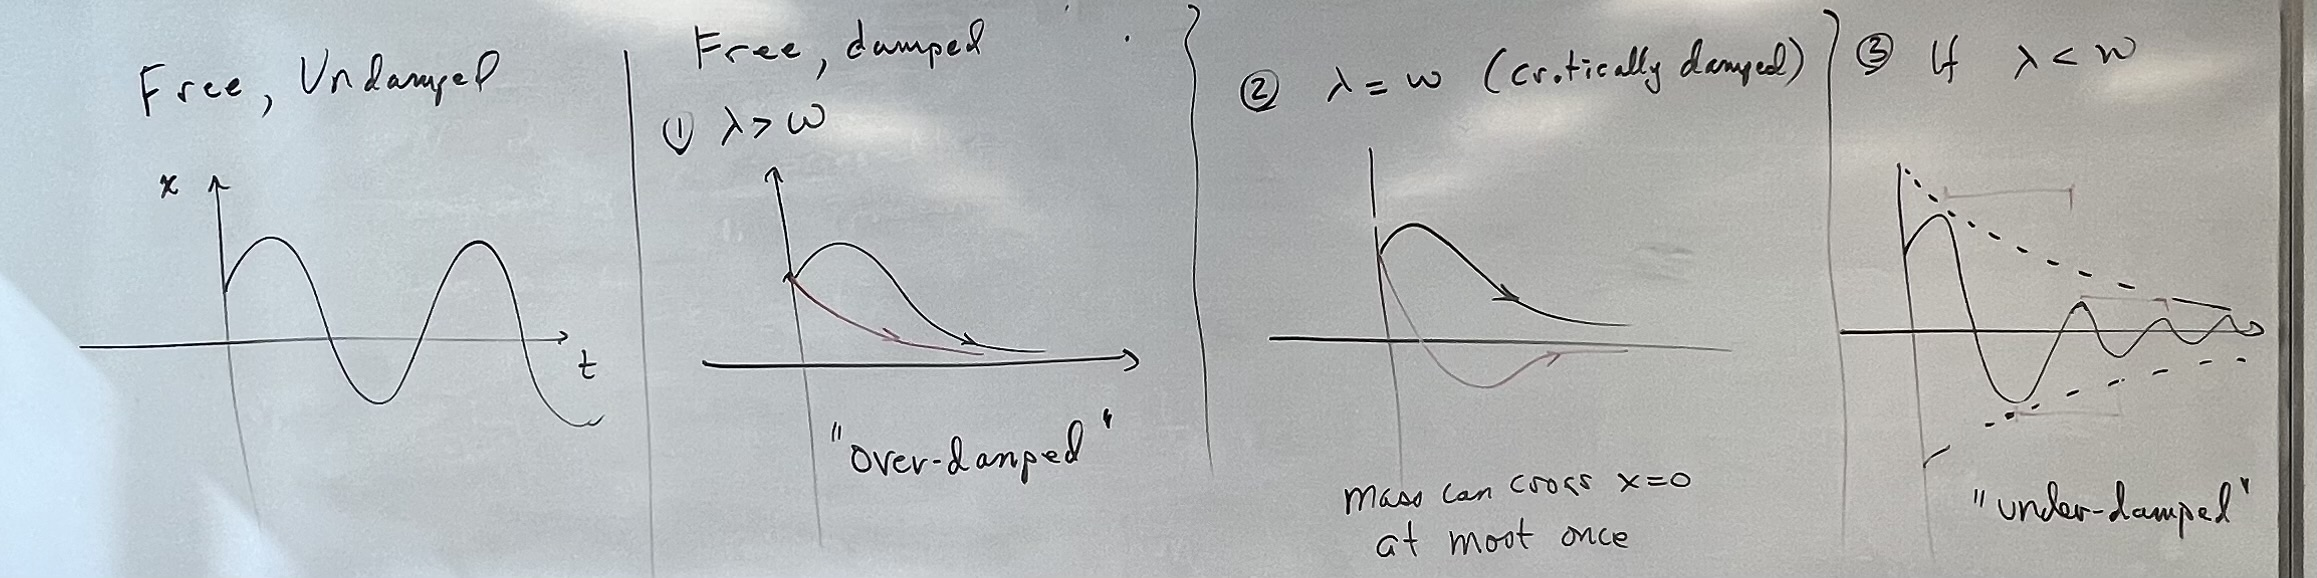
\includegraphics[width=1.2\textwidth,height=3in]{5.1.graphs} % TODO: Make this fit on the sheet
	\caption{Graphs depicting each type of motion of a spring.}
	\label{fig:5.1.graphs}
\end{figure}

\subsection[Driven Motion]{Driven Motion (not Free Motion)}\label{subsec:driven-motion}
Can be both damped or \hyperref[subsubsec:undamped-driven-motion]{undamped}.\\

Imagine the support is oscillating up and down due to an external force.\\\\
If the motion is:
\subsubsection{Undamped}\label{subsubsec:undamped-driven-motion} Assume that $\gamma \neq \omega$
\begin{equation*}
\begin{aligned}
	\frac{d^{2}x}{dt^{2}} + \omega^{2}x &= F(t)\\
										&= F_{0}\sin(\gamma t)\\
\end{aligned}
\end{equation*}

\begin{equation*}
\begin{aligned}
	\frac{d^{2}x}{dt^{2}} + \omega^{2}x &= 0\\
\end{aligned}
\end{equation*}
\begin{equation*}
\begin{aligned}
	& \vdots\\
	x &= c_{1}\cos(\omega t) + c_{2}\sin(\omega t)\\
\end{aligned}
\end{equation*}

\begin{equation*}
\begin{aligned}
	\frac{d^{2}x}{dt^{2}} + \omega^{2}x &= F_{0}\sin(\gamma t)\\
	\hyperref[subsec:method-of-undetermined-coefficients-2]{x_{p}(t)} &= A\cos(\gamma t) + B\sin(\gamma t)\\
	-A\gamma^{2}\cos(\gamma t) - B\gamma^{2}\sin(\gamma t) + \omega^{2}(A\cos(\gamma t) + B\sin(\gamma t)) &= F_{0}\sin(\gamma t)\\
	-A\gamma^{2}\cos(\gamma t) - B\gamma^{2}\sin(\gamma t) + A\omega^{2}\cos(\gamma t) + B\omega^{2}\sin(\gamma t) &= F_{0}\sin(\gamma t)\\
\end{aligned}
\end{equation*}\begin{equation*}
\begin{aligned}
	\cos(\gamma t )\left( -A\gamma^{2} + A\omega^{2} \right) = 0\cos(\gamma t)\sep B(\omega^{2} - \gamma^{2}) = F_{0}\\
	-A\gamma^{2} + A\omega^{2} = 0 \sep B = \frac{F_{0}}{\omega^{2} - \gamma^{2}}\\
	A(\omega^{2} - \gamma^{2}) = 0 \sep B = \frac{F_{0}}{\omega^{2} - \gamma^{2}}\\
	\mbox{ We assumed that } \gamma \neq \omega \mbox{, which forces }&A = 0 \mbox{ for the left equation to work.}\\
	A = 0 \sep B = \frac{F_{0}}{\omega^{2} - \gamma^{2}}\\
\end{aligned}
\end{equation*}

General solution:
\begin{equation}
\begin{aligned}
	x(t) &= x_{c}(t) + x_{p}(t)\\
		 &= c_{1}\cos(\omega t) + c_{2}\sin(\omega t) + \frac{F_{0}}{\omega^{2} - \gamma^{2}}\sin(\gamma t)
\end{aligned}
\end{equation}

If $\gamma$ is almost equal to $\omega$, then $\frac{F_{0}}{\omega^{2} - \gamma^{2}}$ is a large constant. This situation is called Resonance\label{dfn:resonance}.

\example{Driven, Damped, Spring-Mass}
\[ \frac{1}{5}\frac{d^{2}x}{dt^{2}} + 1.2\frac{dx}{dt} + 2x = 5\cos(4t),\ \ x(0)=\frac{1}{2},\ \ x'(0)=0 \]
\begin{equation*}
\begin{aligned}
	\frac{d^{2}x}{dt^{2}} + 6\frac{dx}{dt} + 10x = 25\cos(4t)\\
	\frac{d^{2}x}{dt^{2}} + 2\lambda\frac{dx}{dt} + \omega^{2}x = F(t)\\
\end{aligned}
\end{equation*}
where \[ \lambda = 3, \omega = \sqrt{10}, F(t)=25\cos(4t) \]

For instance, if the mass $= 2$kgs, then the spring constant is $k=20$ and $\beta = 12$.

\[ \sqrt{10} = \sqrt{\frac{k}{m}} \Rightarrow 10 = \frac{k}{m} \Rightarrow 10m = k \Rightarrow k = 10(2) = 20 \]
\[ \beta = 2\lambda m = 2(3)(2) = 6(2) = 12 \]

\subsubsection{To solve the complimentary DE}, guess $x = e^{nt}$
\begin{equation*}
\begin{aligned}
	n^{2}e^{nt} + 6ne^{nt} + 10e^{nt} &= 0\\
	n^{2} + 6n + 10 &= 0\\
\end{aligned}
\end{equation*}\begin{equation*}
\begin{aligned}
	n &= \frac{-b \pm \sqrt{b^{2} - 4ac}}{2a}\\
	  &= \frac{-6 \pm \sqrt{6^{2} - 4(1)(10)}}{2(1)}\\
	  &= \frac{-6 \pm \sqrt{36 - 40}}{2}\\
	  &= \frac{-6 \pm \sqrt{-4}}{2}\\
	  &= \frac{-6 \pm 2i}{2}\\
	  &= -3 \pm i\\
\end{aligned}
\end{equation*}\begin{equation*}
\begin{aligned}
	x_{1} = e^{-3t}\cos(t) \sep x_{2} = e^{-3t}\sin(t)\\
\end{aligned}
\end{equation*}

\subsubsection{To find a particular solution}
Guess
\begin{equation*}
\begin{aligned}
	x_{p} &= A\cos(4t) + B\sin(4t)\\
	x_{p}' &= -4A\sin(4t) + 4B\cos(4t)\\
	x_{p}'' &= -16A\cos(4t) - 16B\sin(4t)\\
\end{aligned}
\end{equation*}
\begin{equation*}
\begin{aligned}
	-16A\cos(4t) - 16B\sin(4t) + 6\left( -4A\sin(4t) + 4B\cos(4t) \right) + 10\left( A\cos(4t) + B\sin(4t) \right) = 25\cos(4t)\\
	-16A\cos(4t) - 16B\sin(4t) - 24A\sin(4t) + 24B\cos(4t) + 10A\cos(4t) + 10B\sin(4t) = 25\cos(4t)\\
	-16A\cos(4t) + 10A\cos(4t) + 24B\cos(4t) - 16B\sin(4t) - 24A\sin(4t) + 10B\sin(4t) = 25\cos(4t)\\
	-6A\cos(4t) + 24B\cos(4t) - 6B\sin(4t) - 24A\sin(4t) = 25\cos(4t)\\
	\cos(4t)(-6A + 24B) + \sin(4t)(-6B - 24A) = 25\cos(4t)\\
\end{aligned}
\end{equation*}

%</Section-5.1-2>

\end{document}